\documentclass{article}
\usepackage{spconf,amsmath,graphicx,hyperref}
\hypersetup{hidelinks}
\usepackage[flushleft]{threeparttable}
\usepackage{cite}
\usepackage{booktabs, multirow}
\usepackage{enumitem} %缩进itemize
\usepackage{amssymb}
\usepackage[table]{xcolor}
\newif\ifshowchanges
% \showchangestrue
\showchangesfalse
\newcommand{\rev}[1]{%
  \ifshowchanges
    \textcolor{red}{#1}%
  \else
    #1%
  \fi
}
\usepackage{pgf}

\definecolor{heatblue}{RGB}{65,115,200}
\definecolor{heatred}{RGB}{205,92,92}

\newcommand{\heatpos}[1]{%
  \pgfmathtruncatemacro{\shadevalue}
    {min(54,14+40*sqrt((#1)/10))}%
  \edef\heatcolor{heatblue!\shadevalue}%
  \expandafter\cellcolor\expandafter{\heatcolor}%
  $+$#1%
}

\newcommand{\heatneg}[1]{%
  \pgfmathtruncatemacro{\shadevalue}
    {min(54,14+40*sqrt((#1)/10))}%
  \edef\heatcolor{heatred!\shadevalue}%
  \expandafter\cellcolor\expandafter{\heatcolor}%
  $-$#1%
}

\newcommand{\heatposbest}[1]{%
  \pgfmathtruncatemacro{\shadevalue}
    {min(54,14+40*sqrt((#1)/10))}%
  \edef\heatcolor{heatblue!\shadevalue}%
  \expandafter\cellcolor\expandafter{\heatcolor}%
  $\mathbf{+}$\textbf{#1}%
}

\newcommand{\heatnegbest}[1]{%
  \pgfmathtruncatemacro{\shadevalue}
    {min(54,14+40*sqrt((#1)/10))}%
  \edef\heatcolor{heatred!\shadevalue}%
  \expandafter\cellcolor\expandafter{\heatcolor}%
  $\mathbf{-}$\textbf{#1}%
}

% \usepackage{lilyglyphs} % dynamic symbols
% \usepackage{tikz}
% \usetikzlibrary{arrows.meta,positioning,fit,calc}
% \tikzset{
%   block/.style={draw, rounded corners, very thick, align=center, inner sep=3pt, minimum height=8mm, fill=white},
%   tinyblock/.style={draw, rounded corners, thick, inner sep=2pt, minimum height=4mm, fill=white},
%   arrow/.style={-Latex, very thick}
% }

% \title{CASM: A Context-Aware Semi-Markov Alternative to DBN Post-Processor for Beat Tracking}
\title{CASM: Context-Aware Semi-Markov Post-Processor for Beat Tracking}

\name{Zhanhong He$^{1,3}$, Hanyu Meng$^{1,3}$, Yaolong Ju$^{1,}$\sthanks{Corresponding author, juyaolong@gbu.edu.cn.}}
\address{
    $^{1}$Great Bay University, Dongguan, China\\
    $^{2}$The University of Western Australia, Perth, Australia\\
    $^{3}$The University of New South Wales, Sydney, Australia
}

\begin{document}
\ninept
\maketitle

\begin{abstract}
At the final stage of beat tracking, neural activations need to be decoded into a discrete, musically coherent event sequence. Direct peak picking follows the local evidence but tends to produce spurious and missed detections. Dynamic Bayesian networks (DBNs), the dominant post-processing approach, suppress such errors by imposing explicit human-specified global assumptions. They work well when predefined tempo and meter assumptions match the music, but expressive or rhythmically complex pieces often depart from them, so the decoder can override correct local evidence instead of correcting errors. We address this limitation by proposing CASM, a model-agnostic, context-aware semi-Markov decoder that exploits local structure in beat activations. CASM estimates local periodicity and ambiguity from the activations, then commits strongly when the cues are clear and relaxes toward the neural output when they are ambiguous, with built-in safeguards keeping this behavior stable and predictable. Using a single configuration, CASM improves F1, CMLt, and AMLt across BeatThis, MSCNN, and TCN models on GTZAN, and delivers state-of-the-art performance on SMC. Under the reported calibration-sensitivity protocol, CASM also exhibits less variation than DBN.\footnote{Code and demo are available at \url{https://zhanh-he.github.io/casm-beat-tracking}.}
\end{abstract}

\begin{keywords}
beat tracking, context-aware, semi-Markov model, post-processing, local periodicity
\end{keywords}


\section{Introduction}
\label{sec:intro}
Beat tracking locates the perceptual pulses that organize musical time, and
downbeat tracking identifies which pulses begin bars. Their outputs support
transcription, structural analysis, synchronization, and interactive music
systems \cite{chiu2023localperiodicity,foscarin2024beat}. Modern trackers usually
produce framewise beat/downbeat activations before a decoder converts them into
events. Direct peak picking stays close to those activations but can leave
missing, duplicated, or metrically inconsistent events; structured decoding can
restore coherence, yet may overwrite correct evidence when its rhythmic
assumptions do not fit the recording.

Sequence models have long addressed this trade-off through dynamic programming,
probabilistic beat extraction, and periodicity filtering
\cite{ellis2007beattracking,korzeniowski2014crf,bock2015combfilter}. DBNs remain a
standard joint decoder: they infer tempo, phase, and meter from the observations,
but do so within globally configured state support and transition laws
\cite{krebs2015dbn,bock2016joint}. A mismatch can therefore force errors on slow,
expressive, or metrically unusual music \cite{foscarin2024beat,ahn2026smcblindspot}.
PLPDP instead obtains a time-varying inter-beat interval and pulse-strength
confidence from PLP and uses them to adapt the target and weight of dense-frame
dynamic programming \cite{chiu2023localperiodicity}. It already makes structure
local and confidence-dependent; what it does not explicitly measure is whether
the selected period clearly defeats its strongest competitor. Differentiable PLP
likewise lets multiple candidate kernels shape the pulse representation
\cite{chiu2025dplp}, so ambiguity handling by itself is not our novelty claim.

We propose Context-Aware Semi-Markov (CASM) decoding for frozen beat/downbeat
activations. CASM estimates a local period and its best-versus-competitor margin,
then uses the two quantities to centre and scale a sparse event-to-event duration
preference. Clear evidence supports regularity; ambiguity weakens and broadens
the preference so that the activations regain influence. This offline path over
retained peaks differs from the causal framewise jump-back model of
\cite{heydari2022semimarkov} and the particle-filter systems BeatNet/BeatNet+
\cite{heydari2021beatnet,heydari2024beatnetplus}, which target online joint rhythm
analysis. A separate count safeguard handles implausible paths, and a
beat-synchronous decoder places downbeats on the selected beat grid.

One validation-selected CASM configuration is frozen across three backbones and
two evaluation corpora, requiring neither backbone retraining nor per-track BPM
or meter settings. Our contribution is a novel and effective offline decoder
whose explicit period-competition signal improves Direct in every reported F1,
CMLt, and AMLt comparison while retaining a transparent, model-agnostic
deployment interface.

\section{Methodology}
\label{sec:method}
\rev{\subsection{CASM Overview}}
\rev{CASM constructs a sparse path over activation-supported peaks and estimates
both local periodicity and its ambiguity. The local period centres a
segment-duration preference, while its margin over the strongest competing
period controls the preference's strength and tolerance. With a clear winner,
CASM can recover weak but activation-supported beats by enforcing local
regularity. With close competitors, it weakens the duration term and lets the
activation evidence dominate. Fig.~\ref{fig:casm-examples} illustrates these two
regimes: the structured path recovers supported events in the left excerpt and,
without triggering the separate count safeguard, coincides with Direct under
ambiguity in the right excerpt. The safeguard returns Direct only when the
complete path is implausibly sparse or dense; a beat-synchronous meter decoder
then keeps downbeats on the selected beat grid.}

\begin{figure}[h!]
\centering

\includegraphics[width=\columnwidth]{figures/p0.jpg}
\vspace{-2mm}
\caption{CASM decisions on held-out BeatThis activations from SMC. A clearly
separated local period supports weak activation peaks (left); competing periods
weaken the duration term until CASM and Direct coincide in this example (right).
DBN and PLPDP are shown for context. Reference beats and IBI are used only for
visual interpretation, not by the decoders.}
\vspace{-4mm}
\label{fig:casm-examples}
\end{figure}
\vspace{-2mm}
\rev{\subsection{Context-aware beat decoding}}

\rev{A frozen tracker produces a beat logit $z_t^{\mathrm b}$ at each
frame $t$, with activation
$a_t=\operatorname{sigmoid}(z_t^{\mathrm b})$ and frame rate $F$.
We retain local maxima above a fixed threshold $\theta_{\mathrm c}$ as
candidates $\mathcal C=\{t_1,\ldots,t_N\}$, assigning each candidate a
clipped evidence score $e_i$. For $i<j$, the elapsed time is
$\Delta_{ij}=(t_j-t_i)/F$, and edge $(i,j)$ is admissible when
$60/\Delta_{ij}$ lies within 30--300 BPM.}

\rev{CASM selects an ordered candidate path
$\pi=(i_1,\ldots,i_K)$, with $i_1<\cdots<i_K$, by maximizing}

\begin{equation}
\rev{
\mathcal S(\pi)
=
\sum_{k=1}^{K} e_{i_k}
-
\sum_{k=2}^{K}D_{i_{k-1},i_k}
}
\label{eq:casm-objective}
\end{equation}

\rev{where $D_{ij}$ is the duration cost between candidates $i$ and $j$.
The two terms respectively reward strong beat evidence and penalize
rhythmically inconsistent intervals. Because each transition scores a
variable-duration interval, CASM has a semi-Markov structure.}

\rev{At candidate $i$, $q_i(\ell)$ denotes the normalized
autocorrelation score at an admissible lag $\ell$ within a window
centred on $t_i$, including a mild fast-tempo prior. The dominant lag
$\ell_i^\star=\arg\max_\ell q_i(\ell)$ gives the local period
$\tau_i=\ell_i^\star/F$. We define the strongest competing hypothesis
outside a $\pm2$-frame neighbourhood as
$q_i^{\mathrm{alt}}
=\max_{\ell:\,|\ell-\ell_i^\star|>2}q_i(\ell)$.
The normalized period-separation margin is}

\begin{equation}
\rev{
c_i =
\operatorname{clip}_{[0,1]}\!\left(
\frac{
q_i(\ell_i^\star)-q_i^{\mathrm{alt}}
}{
|q_i(\ell_i^\star)|+\epsilon_c
}
\right)
}
\label{eq:casm-reliability}
\end{equation}

\rev{where $\epsilon_c>0$ stabilizes the denominator. A large $c_i$
indicates a clearly dominant period, whereas a small value indicates
ambiguity, including half- or double-time alternatives. Thus, $c_i$ is
a deterministic separation margin rather than a calibrated
probability. Both $\tau_i$ and $c_i$ are median-filtered over five
consecutive candidates.}

\rev{For edge $(i,j)$, CASM combines the endpoint estimates as
$\bar{\tau}_{ij}=\sqrt{\tau_i\tau_j}$ and
$c_{ij}=\sqrt{c_i c_j}$. The ambiguity-conditioned constraint strength
is
$w(c)=\lambda c/\{2[\sigma_0+(1-c)\sigma_{\mathrm u}]^2\}$,
giving the duration cost}

\begin{equation}
\rev{
D_{ij}
=
w(c_{ij})\,
\log^2\!\left(
\frac{\Delta_{ij}}{\bar{\tau}_{ij}}
\right)
}
\label{eq:casm-duration}
\end{equation}

\rev{Here, $\lambda>0$ controls the overall penalty strength,
$\sigma_0>0$ sets the minimum timing tolerance, and
$\sigma_{\mathrm u}\geq0$ controls relaxation under ambiguity.
The cost vanishes when $\Delta_{ij}=\bar{\tau}_{ij}$; a large $c_{ij}$
enforces rhythmic regularity, while a small $c_{ij}$ relaxes the
constraint. CASM can therefore recover weak but rhythmically supported
beats without forcing an unreliable tempo grid.}

\rev{Figure~\ref{fig:casm-response} shows how Eq.~\eqref{eq:casm-duration} converts the local period-separation margin into an input-dependent timing constraint. Panel (a) shows the fixed response, panel (b) maps transitions from different datasets and backbones onto it, and panel (c) summarizes the resulting track-level
constraint strengths. Thus, one frozen CASM configuration adapts its
constraint across inputs. The figure illustrates decoder conditioning,
not tracking accuracy; the direct fallback is a separate safeguard.}

\begin{figure}[h!]
\centering
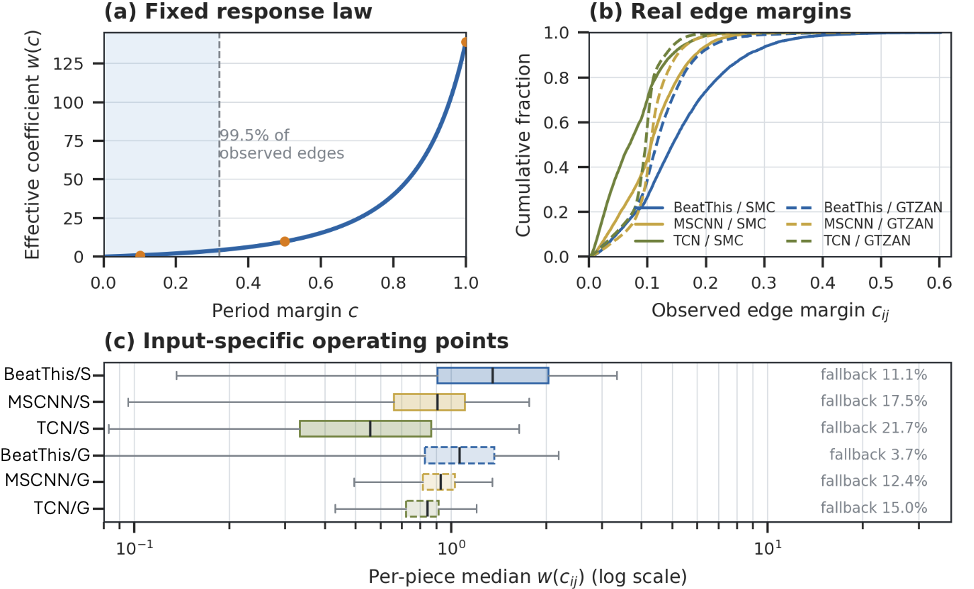
\includegraphics[width=\columnwidth]{figures/p1.jpg}
\vspace{-2mm}
\caption{Input-conditioned duration stiffness under one frozen CASM
configuration. (a) Fixed constants map period margin $c$ to coefficient $w(c)$;
shading contains 99.5\% of observed structured-path edges. (b) Margin
distributions differ across backbones and corpora. (c) Per-piece median
coefficients consequently occupy different operating ranges; annotations report
the separate count-ratio fallback rate. The fixed parameters define one response
law, not one effective rigidity for every input.}
\vspace{-4mm}
\label{fig:casm-response}
\end{figure}
\vspace{-3mm}
\rev{\subsection{Safeguards and downbeat decoding}}
\rev{A Viterbi-style dynamic program maximizes
Eq.~\eqref{eq:casm-objective} and backtracks the best beat path, allowing
a restart after an unfavourable prefix. As a safeguard, CASM also forms
a direct fallback path using seven-frame max pooling, a zero-logit
threshold, and one-frame deduplication
\cite{foscarin2024beat}. If
$\lvert\pi_{\mathrm{CASM}}\rvert/
 \lvert\pi_{\mathrm{direct}}\rvert
 \notin[r_{\min},r_{\max}]$,
indicating an implausibly sparse or dense CASM path, the direct path is
returned. This rule is deterministic and requires no learned router.}

\rev{Downbeats are decoded on the selected beat grid using a second
dynamic program that favours valid bar lengths and discourages
unnecessary meter changes. If its output strongly disagrees with the
direct downbeat activations snapped to the same grid, the snapped result
is used, ensuring that every downbeat coincides with an output beat.
All scalar parameters are calibrated once on the development folds and
then frozen across tracks, datasets, and backbone models. Inference
requires no reference annotations, externally supplied BPM or meter,
per-track tuning, or learned decoder parameters.}

\section{Experiments}
\label{sec:exp}
\subsection{Evaluation protocol}
\textbf{Datasets and splits.} We use the publicly released data from BeatThis \cite{foscarin2024beat}, which contains 4,556 tracks from 18 beat-tracking datasets, including SMC, Hainsworth, Ballroom, Beatles, and others. This data collection provides preprocessed log-Mel spectrograms computed from 22.05kHz mono audio at 50 fps, together with a fixed eight-fold partition to conduct cross-validation experiments. For each fold, the corresponding backbone checkpoint is trained on the remaining seven folds, ensuring that evaluated tracks remain unseen during training. Among these datasets, SMC provides beat but not downbeat annotations, and is widely recognized as the hard one compared to the others. Additionally, GTZAN provides 993 tracks as the held-out evaluation set, which is excluded from the cross-validation pool.

\textbf{Backbones.} We select three models whose implementations are publicly available and readily reproducible. For BeatThis, we use the original code and pretrained checkpoints \cite{foscarin2024beat}. MSCNN is adapted from the multi-scale, multi-task convolutional network of \cite{he2026dynest}, which was designed for 60s Bark-scale specific-loudness features. We modify it to accept the 30s the unified log-Mel input and remove the task heads unrelated to beat and downbeat tracking. TCN was introduced by \cite{bock2020deconstruct}, and we use the re-implementation distributed with \cite{he2026dynest}, which has been adapted from its original 5\,s input to the same 30\,s log-Mel input, with the tempo task head removed. All resulting backbones are trained on the same data and frozen before decoding performance comparison, ensuring that every post-processor receives exactly the same 50\,Hz framewise beat/downbeat activations from a given backbone.

\textbf{Evaluation.} Following previous work \cite{foscarin2024beat}, the eight fold-specific checkpoints of each backbone are evaluated on GTZAN and their corresponding out-of-fold SMC partitions, with scores macro-averaged over total evaluation. We use \texttt{mir\_eval} to compute F1 score with a $\pm70$\,ms tolerance, CMLt, and AMLt \cite{raffel2014mireval}. CMLt measures continuity at the correct metrical level, whereas AMLt additionally accepts standard off-beat and half- or double-level interpretations.

\subsection{Post-processors and tempo support}
Because CASM targets offline decoding, it may use future context when estimating
local periodicity and selecting the global event path. We compare it with Direct
and the offline post-processors DBN \cite{krebs2015dbn}, PLPDP
\cite{chiu2023localperiodicity}, CombFilter \cite{bock2015combfilter}, and CRF
beat detection \cite{korzeniowski2014crf}. Direct is the peak-picking path defined
in Sec.~\ref{sec:method}, and CASM uses fixed 30--300-BPM support. PLPDP,
CombFilter, and CRF are run with their released/default parameters. For methods
without a joint beat/downbeat decoder, downbeats are decoded from the downbeat
activation stream and snapped to the corresponding beat grid.

DBN receives separate treatment because its behaviour is particularly sensitive to global tempo support. We use the standard joint \texttt{madmom} configuration \cite{krebs2015dbn}: meters $\{3,4\}$, transition weight 100, observation weight 16, threshold 0.05, and the default 55--215-BPM range. Because SMC includes many annotated tempi below 55 BPM \cite{ahn2026smcblindspot}, Table~\ref{tab:postprocessor_ablation} also explores a 30--300-BPM DBN variant in which only the tempo range is changed. For a matched diagnostic, we additionally report CASM with its support restricted to 55--215 BPM on BeatThis activations, with all other CASM settings held fixed.

\subsection{CASM calibration}
CASM has no learned weights or random seed. The final configuration used in all main tables is calibrated once on the union of SMC folds 1--7 (7F) and then frozen for every track, backbone, and dataset. The same global scalar settings are therefore used on BeatThis, MSCNN, and TCN, on both SMC and GTZAN, without per-track or per-dataset BPM, meter, or parameter tuning at inference. Because the aggregate SMC results use eight-fold out-of-fold backbone activations while the decoder configuration is calibrated on folds 1--7, they are out-of-fold with respect to backbone training but are not a nested estimate of decoder calibration.

We analyse calibration-data sensitivity separately rather than using it to choose the main operating point. SMC fold 0 is held out from decoder calibration throughout. From folds 1--7, we enumerate every 1-, 2-, and 4-fold calibration subset ($7$, $21$, and $35$ combinations) and the seven-fold union. For both CASM and DBN, a decoder configuration is selected independently on each calibration subset and then evaluated on the same fixed SMC-fold-0 panel and on GTZAN using one fixed backbone seed. The resulting distributions therefore measure sensitivity to the amount and composition of calibration data, while the 7F CASM configuration is the maximally supported global configuration used for the main results.
\section{Results}
\label{sec:results}

\subsection{Comparison with post-processors}

\begin{table}[t]
\centering
\caption{Comparison with post-processing methods on fixed backbone activations. DBN default uses 55--215 BPM, while wide-support variants use 30--300 BPM to cover low-tempo SMC tracks \cite{ahn2026smcblindspot}, all other settings are unchanged.}
\label{tab:postprocessor_ablation}
\begingroup
\fontsize{7.5pt}{8.5pt}\selectfont
\setlength{\tabcolsep}{0.7pt}
\renewcommand{\arraystretch}{0.92}
\resizebox{\columnwidth}{!}{%
\begin{tabular}{l|c|rrr@{\hspace{2pt}}|rrr@{\hspace{2pt}}|rrr}
\toprule
\multicolumn{1}{c|}{\multirow{2}{*}{\textbf{Method}}}
& \multicolumn{1}{c|}{\multirow{2}{*}{\textbf{BPM}}}
& \multicolumn{6}{c|}{\textbf{GTZAN (Beat / Downbeat)}}
& \multicolumn{3}{c}{\textbf{SMC (Beat)}} \\
\cmidrule(lr){3-8}
\cmidrule(l){9-11}
& & F1 & CMLt & AMLt
& F1 & CMLt & AMLt
& F1 & CMLt & AMLt \\
\midrule

\textbf{BeatThis} (direct) \cite{foscarin2024beat}
& --
& 89.1 & 79.8 & 89.8
& 78.3 & 67.2 & 79.1
& 62.7 & 51.4 & 61.0 \\

w. CASM
& 30-300
& \heatposbest{0.3} & \heatposbest{0.8} & \heatpos{1.2}
& \heatposbest{0.7} & \heatpos{3.6} & \heatpos{8.0}
& \heatposbest{0.3} & \heatposbest{2.4} & \heatposbest{3.6} \\

w. CASM, ablation
& 55-215
& \heatpos{0.1} & \heatpos{0.5} & \heatpos{0.6}
& \heatpos{0.5} & \heatpos{2.9} & \heatpos{5.8}
& \heatpos{0.1} & \heatpos{0.4} & \heatpos{2.0} \\

w. DBN \cite{krebs2015dbn}
& 30-300
& \heatneg{0.5} & \heatneg{0.9} & \heatpos{0.2}
& \heatneg{1.5} & \heatneg{0.6} & \heatpos{1.1}
& \heatneg{1.6} & \heatpos{0.4} & \heatpos{3.5} \\

w. DBN, default
& 55-215
& \heatneg{1.0} & \heatpos{0.7} & \heatpos{1.3}
& \heatneg{0.9} & \heatposbest{6.2} & \heatposbest{8.7}
& \heatneg{5.2} & \heatneg{3.9} & \heatpos{1.5} \\

% w. PLPDP
% & 55--215
% & \heatneg{0.1} & \heatposbest{0.8} & \heatpos{0.1}
% & \heatneg{0.2} & \heatpos{0.1} & \heatneg{0.1}
% & \heatneg{1.4} & \heatneg{4.7} & \heatpos{0.5} \\

w. PLPDP \cite{chiu2023localperiodicity}
& 30-300
& \heatpos{0.1} & \heatpos{0.3} & \heatpos{0.3}
& \heatpos{0.1} & \heatpos{0.2} & \heatpos{0.2}
& \heatneg{0.9} & \heatneg{3.5} & \heatneg{0.3} \\

w. CombFilter \cite{bock2015combfilter}
& 30-300
& \heatneg{4.0} & \heatneg{3.6} & \heatpos{0.1}
& \heatneg{3.3} & \heatpos{3.2} & \heatpos{7.6}
& \heatneg{7.1} & \heatpos{1.1} & \heatpos{3.1} \\

w. CRF \cite{korzeniowski2014crf}
& 30-300
& \heatneg{0.6} & \heatneg{0.3} & \heatposbest{1.4}
& \heatneg{1.4} & \heatpos{1.9} & \heatpos{5.5}
& \heatneg{1.2} & \heatpos{1.4} & \heatpos{1.2} \\

\midrule
\textbf{MSCNN} (direct) \cite{he2026dynest}
& --
& 86.1 & 73.4 & 79.9
& 70.8 & 53.1 & 63.1
& 57.2 & 42.0 & 48.4 \\

w. CASM
& 30--300
& \heatposbest{0.4} & \heatpos{1.6} & \heatpos{2.4}
& \heatpos{1.5} & \heatpos{12.5} & \heatpos{18.3}
& \heatposbest{0.3} & \heatposbest{3.5} & \heatposbest{6.8} \\
w. DBN
& 30--300
& \heatneg{1.1} & \heatpos{0.2} & \heatpos{5.9}
& \heatneg{0.9} & \heatpos{9.5} & \heatpos{14.6}
& \heatneg{0.2} & \heatpos{2.2} & \heatpos{4.1} \\
w. DBN, default
& 55--215
& \heatneg{0.6} & \heatposbest{4.0} & \heatposbest{7.2}
& \heatposbest{1.8} & \heatposbest{15.8} & \heatposbest{21.2}
& \heatneg{4.9} & \heatpos{0.3} & \heatpos{3.9} \\
\midrule

\textbf{TCN} (direct) \cite{bock2020deconstruct}
& --
& 87.1 & 73.8 & 81.7
& 62.4 & 24.6 & 59.9
& 52.9 & 30.1 & 36.0 \\
w. CASM
& 30--300
& \heatposbest{0.3} & \heatposbest{1.3} & \heatpos{1.6}
& \heatpos{2.1} & \heatpos{9.2} & \heatpos{13.4}
& \heatposbest{1.7} & \heatposbest{4.5} & \heatposbest{8.2} \\
w. DBN
& 30--300
& \heatneg{1.9} & \heatneg{0.8} & \heatpos{4.4}
& \heatneg{0.2} & \heatpos{8.9} & \heatpos{9.3}
& \heatneg{0.4} & \heatpos{2.1} & \heatpos{5.9} \\
w. DBN, default
& 55--215
& \heatneg{2.6} & \heatneg{0.7} & \heatposbest{5.0}
& \heatposbest{4.9} & \heatposbest{23.2} & \heatposbest{22.9}
& \heatneg{0.9} & \heatneg{7.0} & \heatpos{2.3} \\
% w. CombFilter
% & --
% & \heatneg{6.3} & \heatpos{1.1} & \heatpos{4.3}
% & \heatneg{2.2} & \heatpos{12.2} & \heatpos{19.5}
% & \heatneg{5.7} & \heatpos{9.3} & \heatpos{17.9} \\
% w. CRF
% & --
% & \heatpos{0.7} & \heatpos{3.3} & \heatpos{7.8}
% & \heatpos{1.5} & \heatpos{4.8} & \heatpos{18.3}
% & \heatneg{2.3} & \heatneg{2.2} & \heatpos{12.4} \\
\bottomrule
\end{tabular}%
}
\endgroup
\end{table}

Table~\ref{tab:postprocessor_ablation} isolates the post-processor by holding the backbone activations fixed. With 30--300-BPM support, the CASM improves BeatThis (direct pick-peaking) on every reported F1, CMLt, and AMLt entry across all three backbones and both datasets. Relative to DBN, CASM generally preserves F1 better, while DBN can produce larger continuity gains, particularly for GTZAN downbeats. The large SMC change between the 55--215- and 30--300-BPM DBN variants also shows how strongly a fixed DBN can depend on its global tempo range. PLPDP, CombFilter, and CRF provide useful alternatives, but none improves every reported metric under the same fixed activations. Overall, CASM gives a conservative F1--continuity operating point that transfers across backbone families without changing decoder parameters.

\subsection{Comparison with the state of the art}

\begin{table}[t]
\centering
\caption{Comparison with recent beat-tracking systems. BeatThis (direct) and CASM results were obtained from our experiments, while all other values are reported from their original papers.}
\label{tab:audiodyn_cross_dataset_sota}
\begingroup
\fontsize{8pt}{11pt}\selectfont
\setlength{\tabcolsep}{0.5pt}
\renewcommand{\arraystretch}{1.0}
\resizebox{\columnwidth}{!}{%
\begin{tabular}{l|ccc|ccc|ccc}
\toprule
\multicolumn{1}{c|}{\multirow{2}{*}{\textbf{Method}}}
& \multicolumn{6}{c|}{\textbf{GTZAN (Beat / Downbeat)}}
& \multicolumn{3}{c}{\textbf{SMC (Beat)}} \\
\cmidrule(lr){2-4}
\cmidrule(lr){5-7}
\cmidrule(l){8-10}
& F1 & CMLt & AMLt
& F1 & CMLt & AMLt
& F1 & CMLt & AMLt \\
\midrule
\rowcolor{gray!10}
\textbf{HN-MERT} w. DBN \cite{ru2025hingenet}
& \textbf{89.7} & 81.4 & \textbf{94.3}
& 77.4 & 71.6 & 87.2
& 61.7 & -- & -- \\
\textbf{HN-MusicFM} w. DBN
& 89.2 & 80.9 & 93.7
& \textbf{79.8} & 73.2 & \textbf{89.5}
& 60.6 & -- & -- \\
\rowcolor{gray!10}
\textbf{BeatFM-MERT} w. DBN \cite{ru2025beatfm}
& \underline{89.5} & \underline{82.7} & \underline{93.9}
& 76.7 & 70.2 & 85.4
& 61.3 & -- & -- \\
\textbf{BeatFM-MusicFM} w. DBN
& 89.1 & 80.6 & 93.5
& \underline{79.6} & \underline{74.4} & \underline{88.7}
& 60.5 & -- & -- \\
% \textbf{SpecTNT-TCN} w. DBN \cite{hung2022modeling}
% & 88.7 & 81.2 & 92.0
% & 75.6 & 71.5 & 88.1
% & 60.5 & 51.4 & 66.3 \\
% \textbf{TCN} + DBN  \cite{bock2020deconstruct}
% & 88.5 & 81.3 & 93.1
% & 67.2 & 64.0 & 83.2
% & 55.2 & 46.5 & 64.3 \\
\rowcolor{gray!10}
\textbf{BeatMamba} w. DBN \cite{ru2026beatmamba}
& 88.9 & 82.3 & \textbf{94.3}
& -- & -- & --
& 58.7 & 46.8 & 62.4 \\
\textbf{BeatKAN} w. DBN \cite{zhang2025beatkan}
& 88.2 & 78.1 & 92.3
& -- & -- & --
& 59.8 & 48.4 & 64.0 \\
\rowcolor{gray!10}
\textbf{MDM-BeatThis} (direct) \cite{foscarin2026masked}
& \textbf{89.7} & \textbf{82.9} & 92.5
& 79.5 & \textbf{76.4} & 88.5
& 61.0 & 48.9 & \underline{64.3} \\
\midrule
\textbf{BeatThis} (direct) \cite{foscarin2024beat}
& 89.1 & 79.8 & 89.8
& 78.3 & 67.2 & 79.1
& \underline{62.7} & \underline{51.4} & 61.0 \\
% \textbf{BeatThis} w. DBN (default \& opt)
% & 88.1 & 80.5 & 91.1
% & 77.4 & 73.4 & 87.8
% & 57.5 & 47.5 & 62.5 \\
\rowcolor{gray!10}
\textbf{BeatThis} w. CASM
& 89.4 & 80.6 & 91.0
& 79.0 & 70.8 & 87.1
& \textbf{63.0} & \textbf{53.8} & \textbf{64.6} \\
\bottomrule
\end{tabular}%
}
\endgroup
\end{table}

Table~\ref{tab:audiodyn_cross_dataset_sota} compares the BeatThis works with CASM results with recent literature. While using CASM improves six beat/downbeat metrics compared to BeatThis (directly peak-picking) on the GTZAN, we reported the highest scores on SMC compared to the other SOTA systems. On GTZAN, stronger task-specific or pre-trained frontends retain the best individual scores. The literature table therefore provides system-level context; controlled claims about decoder behaviour come from Table~\ref{tab:postprocessor_ablation}, where the backbone activations are held fixed.

\subsection{Sensitivity to calibration data}
The sensitivity experiment keeps the evaluation panels fixed and changes only the data used to calibrate the decoder. For each calibration scale $k\in\{1,2,4,7\}$, CASM and DBN are calibrated on the corresponding SMC fold subsets described in Sec.~\ref{sec:exp}, and every selected configuration is evaluated on the same held-out SMC fold 0 and the same GTZAN backbone seed. Thus, the spread at a given scale measures dependence on which calibration folds were used, while the movement of the distribution centre measures how additional calibration data changes transfer to the two fixed evaluation panels.

\begin{figure}[t]
\begin{center}
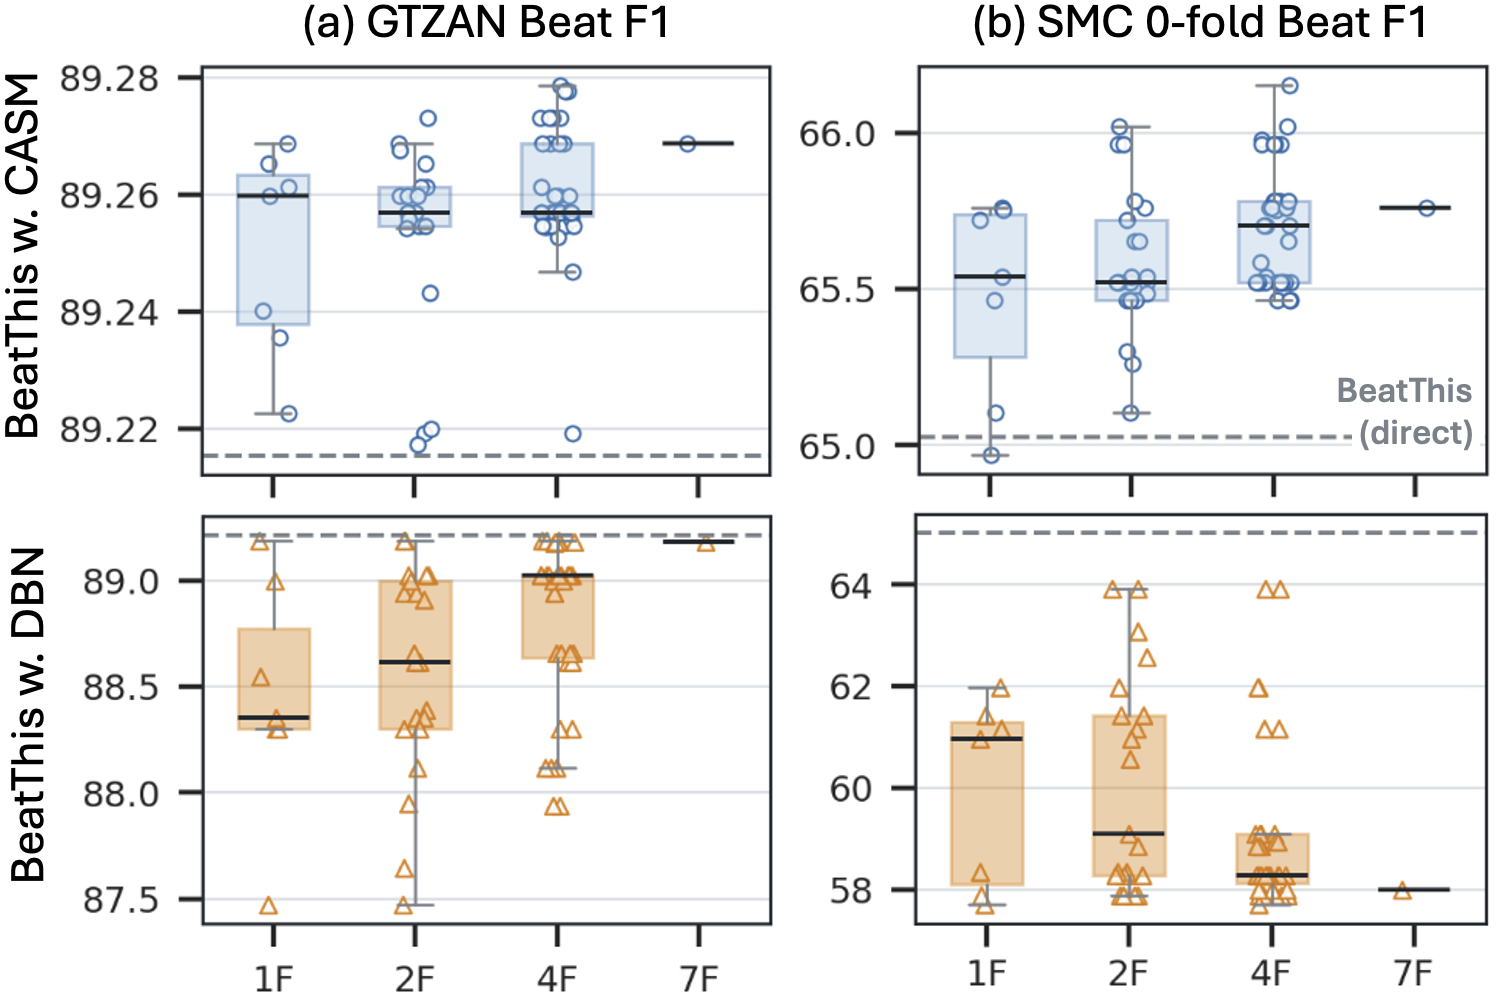
\includegraphics[width=0.9\columnwidth]{figures/p2.jpg}
\caption{Sensitivity to calibration data for CASM and DBN. Each point corresponds to a decoder configuration selected from one of the $7/21/35$ exhaustive 1-/2-/4-fold subsets of SMC folds 1--7 and evaluated on fixed SMC-fold-0 and GTZAN panels; 7F is a single configuration. Boxes are descriptive because calibration subsets overlap, and dashed lines show Direct performance.}
\label{fig:calibration-scale}
\end{center}
\end{figure}

Fig.~\ref{fig:calibration-scale} shows a clear difference in calibration behaviour. CASM remains tightly clustered across fold combinations, and its central performance improves consistently as more calibration folds are used on both the held-out SMC panel and GTZAN. In contrast, DBN exhibits much wider variation across calibration subsets, and the trends on SMC and GTZAN do not move together: configurations favoured by one panel can transfer poorly to the other. This cross-dataset disagreement is consistent with stronger calibration-set over-specialisation in the fixed DBN parameterisation. The 7F CASM setting used in the main tables is therefore supported by the full available calibration pool rather than selected from a favourable smaller-fold combination.

\section{Conclusion and Future Work}
\label{sec:concl}

CASM revisits structured beat decoding as an inductive bias conditioned on each input, not as a return to a fixed global grid. It joins activation-supported events with locally centred segment potentials and deliberately relaxes those potentials when periodic evidence is ambiguous. Once globally calibrated, the same deterministic module runs without upstream retraining, user annotation, or per-track tempo and meter settings. Current evidence supports a conservative F1--continuity alternative to Direct and DBN decoding, not universal dominance. The next version should use strict nested or leave-one-dataset-out calibration, matched tempo-support baselines, PLPDP and mechanism ablations, and explicit safeguard statistics. Multi-hypothesis period paths, causal decoding, and a differentiable duration layer are natural extensions, as is evaluation on every recent tracker that releases compatible activations.

\bibliographystyle{IEEEbib}
\bibliography{casm}

\end{document}
